%%%%%%%% ICML 2021 EXAMPLE LATEX SUBMISSION FILE %%%%%%%%%%%%%%%%%

\documentclass{article}

\usepackage{microtype}
\usepackage{graphicx}
\usepackage{subfigure}
\usepackage{booktabs} % for professional tables
\usepackage{hyperref}
% the following package enables the use of multiline comments:
\usepackage{comment}

% Attempt to make hyperref and algorithmic work together better:
\newcommand{\theHalgorithm}{\arabic{algorithm}}

% Use the following line for the initial blind version submitted for review:
%\usepackage{icml2021}

% If accepted, instead use the following line for the camera-ready submission:
\usepackage[accepted]{icml2021}

% The \icmltitle you define below is probably too long as a header.
% Therefore, a short form for the running title is supplied here:
\icmltitlerunning{Board games group recomendation using metadata}

\begin{document}

\twocolumn[
    \icmltitle{Board games group recomendation using metadata}

    % It is OKAY to include author information, even for blind
    % submissions: the style file will automatically remove it for you
    % unless you've provided the [accepted] option to the icml2021
    % package.

    % List of affiliations: The first argument should be a (short)
    % identifier you will use later to specify author affiliations
    % Academic affiliations should list Department, University, City, Region, Country
    % Industry affiliations should list Company, City, Region, Country

    % You can specify symbols, otherwise they are numbered in order.
    % Ideally, you should not use this facility. Affiliations will be numbered
    % in order of appearance and this is the preferred way.
    \icmlsetsymbol{equal}{*}

    \begin{icmlauthorlist}
        \icmlauthor{Eduardo Salinas}{to}
        \icmlauthor{Alfonso Badilla}{to}
        \icmlauthor{Nicolás Gutiérrez}{to}
    \end{icmlauthorlist}

    \icmlaffiliation{to}{Department of Computation, Pontificia Universidad Católica de Chile, Santiago, Chile}

    \icmlcorrespondingauthor{Eduardo Salinas}{esalinasbarros@uc.cl}
    \icmlcorrespondingauthor{Alfonso Badilla}{alfonso.badilla@uc.cl}
    \icmlcorrespondingauthor{Nicolás Gutiérrez}{njgutierrez@uc.cl}

    % You may provide any keywords that you find helpful for describing your paper; these are used to populate the "keywords" metadata in the PDF but will not be shown in the document
    \icmlkeywords{Machine Learning, ICML, Group recommendation, Metadata}

    \vskip 0.3in
]

% this must go after the closing bracket ] following \twocolumn[ ...

% This command actually creates the footnote in the first column
% listing the affiliations and the copyright notice.
% The command takes one argument, which is text to display at the start of the footnote.
% The \icmlEqualContribution command is standard text for equal contribution.
% Remove it (just {}) if you do not need this facility.

\printAffiliationsAndNotice{} % otherwise use the standard text.

\begin{abstract}
    In this document we propose a group recommendation system for board games using data from the Board Game Geek website, which includes attributes such as the number of players, average playtime, complexity, and user ratings.
    % todo: agregar explicación groso modo del algoritmo
    The implementation employs Python and the scikit-learn library, offering an efficient and scalable solution for group-based game recommendations.
\end{abstract}

\section{Motivation and state of the art}

Board games have been a popular form of entertainment for centuries, and their popularity has only increased in recent years. Even as digital games have become more prevalent, board games have remained a favorite pastime for many people, and the market for board games has grown significantly giving rise to plataforms such as Board Game Geek\footnote{\cite{boardgamegeek}} (BGG). This website is a popular platform for board game enthusiasts, where users can rate and review games, as well as access information about them.

\subsection{State of the art and related work}

This plataform has a vast amount of data that has been used in the past to create recommendation systems. For example,
github user richengo \yrcite{richengo2024} proposed a recommendation system for board games based on user ratings, using a collaborative filtering approach. However, this approach does not take into account the characteristics of many of the games, that are supposed to be played in groups. As such, we propose a group recommendation system to make recommendations tailored to groups of players.

Another example of group recommendation systems is the work of \cite{group_recommenders_repo}, who proposed a group recommendation system for tourism and movies\footnote{This work is hosted on a github repo and is intended to be used as a basic tutorial.}.
This system uses regular clustering algorithms to group users based on their ratings, such as user k-nearest, item k-nearest and support vector decomposition (SVD), and then recommends movies and touristic locations based on the preferences of the group.

\subsection{Proposal}

We propose a refined version of that last system, using metadata-centric clustering to group board games based on their characteristics, and then recommending games to groups of players based on their summed preferences used the functions detailed on the previous work. This system is designed to be more accuarate than the previous one, as it takes into account the characteristics of the games, and not just the ratings of the users.

\section{Data analysis}

The dataset that will be used for this project\footnote{\cite{board_games_kaggle}}, obtained from the website kaggle, has 10 different files, each one tith different information about board games. The main file is \texttt{user\_ratings.csv}, which contains 19 million rows. Due to the limited processing power of Google Collab and our own local machines, we will use a reduced set of items and users for this work. The other files are:

\begin{itemize}
    \item \texttt{games.csv}: This file contains 22 attributes about the rated games and includes 22,000 different games. Among the attributes, we have aspects such as the game description, which could be evaluated using language models, the year of publication (which distributes as shown in figure \ref{fig:publishYear}), the average rating received, among others.
    \item \texttt{ratings\_distribution.csv}: Contains the total ratings for each board game. In general, these ratings distribute as shown in figure \ref{fig:distribucionRatings}.
    \item \texttt{temes.csv}: Contains the themes of each game as a binary flag. The 50 most common themes can be seen in the graph in figure \ref{fig:tematicasComunes}.
    \item \texttt{mechanics.csv}: Contains the game mechanics as a binary flag. The 50 most common mechanics can be seen in the graph in figure \ref{fig:mecanicasComunes}.
    \item \texttt{subcategories.csv}: Contains the subcategories of each game in binary flag format.
    \item \texttt{artists\_reduced.csv}: Contains information about which artist created a certain game in binary flag format. Only artists with more than 3 games created will be considered.
    \item \texttt{designer\_reduced.csv}: Contains information about which designer designed a certain game in binary flag format. Only designers with more than 3 games created are considered.
    \item \texttt{publishers\_reduced.csv}: Contains information about the companies that sell these games in binary flag format. Only companies that sell more than 3 games are considered.

\end{itemize}

\begin{figure}
    \centering
    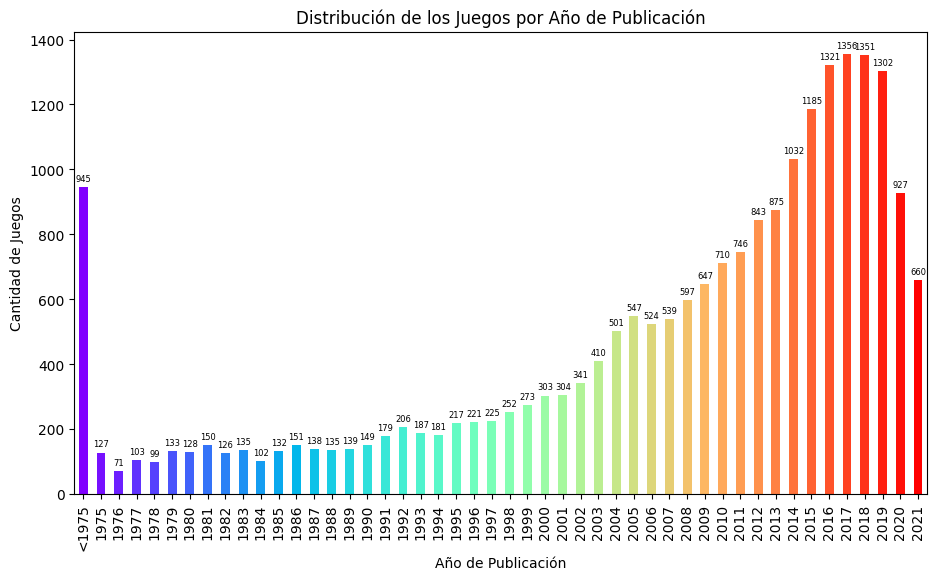
\includegraphics[width=0.8\linewidth]{publishYear.png}
    \caption{Juegos por año de publicación}
    \label{fig:publishYear}
\end{figure}

\begin{figure}[h]
    \centering
    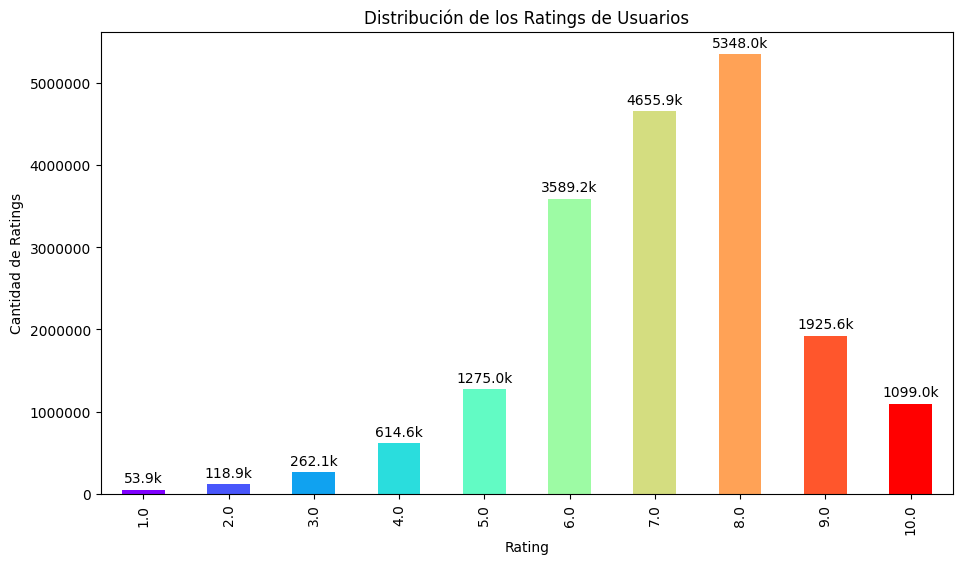
\includegraphics[width=0.8\linewidth]{distribucionRatings.png}
    \caption{Distribución de ratings de juegos}
    \label{fig:distribucionRatings}
\end{figure}

\begin{figure}[h]
    \centering
    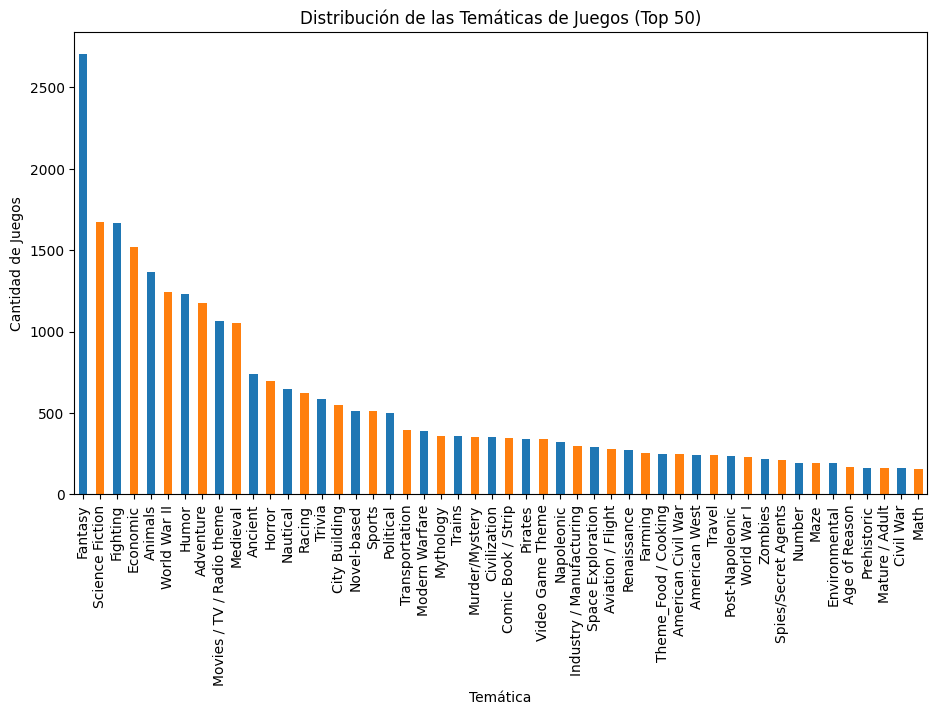
\includegraphics[width=0.8\linewidth]{tematicasComunes.png}
    \caption{Temáticas más comunes en el dataset}
    \label{fig:tematicasComunes}
\end{figure}

\begin{figure}[h]
    \centering
    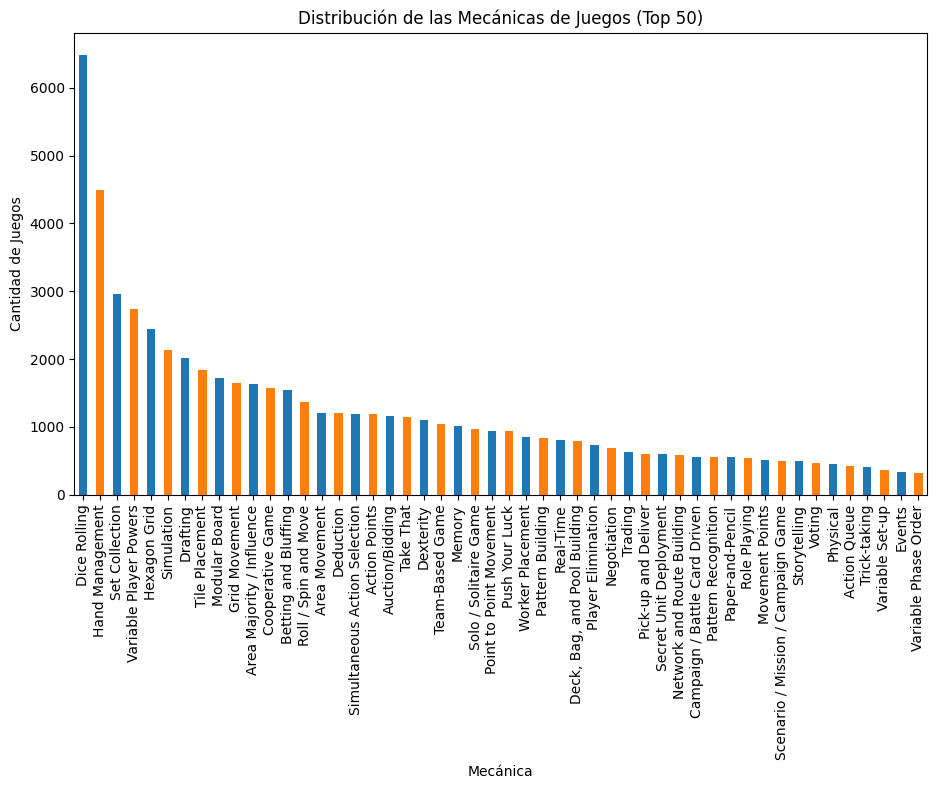
\includegraphics[width=0.8\linewidth]{mecanicasComunes.png}
    \caption{Mecánicas más comunes en el dataset}
    \label{fig:mecanicasComunes}
\end{figure}

\section{Methodology}

The methodology for this project is divided into three main stages: data preprocessing, group making, and recommendation.

\subsection{Data preprocessing}
The first stage consists of reducing the dataset by not picking items without interactions and then dividing the...

% Mostrar gráfico de las clases de usuarios y clases de ítems, además de mostrar cuantos no valen la pena.

\subsection{Group making}

% Insertar referencia y citar apropiadamente el trabajo.
The second stage consists of grouping the users based on their characteristics by using a correlation matrix. The function used is an adaptation of the one used in the "" work, which is based on the cosine similarity between the users. The function is as follows:

% Arreglar función
\begin{equation}
    %\text{similarity}(u, v) = \frac{\sum_{i=1}^{n} u_i \cdot v_i}{\sqrt{\sum_{i=1}^{n} u_i^2} \cdot \sqrt{\sum_{i=1}^{n} v_i^2}}
\end{equation}


\subsection{Recommendation}
The third stage consists of recommending games to groups of players based on their preferences. Since the recommendations are supposed to be made to groups, the preferences of the group are calculated using a variety of methods, that can be described as follows:
\begin{enumerate}
    \item Simple average: The preferences of the group are calculated as the simple average of the preferences of the individual players.
    \item Least misery: The preferences of the group are calculated as the minimum of the preferences of the individual players.
    \item ... % asegurarse que esto está al día con lo que presentemos al final del trabajo
\end{enumerate}

\section{Results}

To evaluate the results of our model, we will compare it to most popular as a sanity check, to iknn applied to the same dataset and to SVD applied to the same dataset. % Agregar AGREE si logramos hacerlo funcionar ahora que tenemos menos datos. 

The metrics that will be used to evaluate the performance of each model are the following:

\begin{itemize}
    \item Precision at k: This metric measures the proportion of recommended items that are relevant to the user, where relevance is defined as the items that the user has interacted with.
    \item Recall at k: This metric measures the proportion of relevant items that are recommended to the user.
    \item F1 score: This metric is the harmonic mean of precision and recall, and is used to measure the overall performance of the model.
\end{itemize}


\section{Sensitivity Analysis}

\section{Conclusions}

% You can use footnotes\footnote{Footnotes should be complete sentences.} to provide readers with additional information about a topic without interrupting the flow of the paper.

% \begin{figure}[ht]
% \vskip 0.2in
% \begin{center}
% \centerline{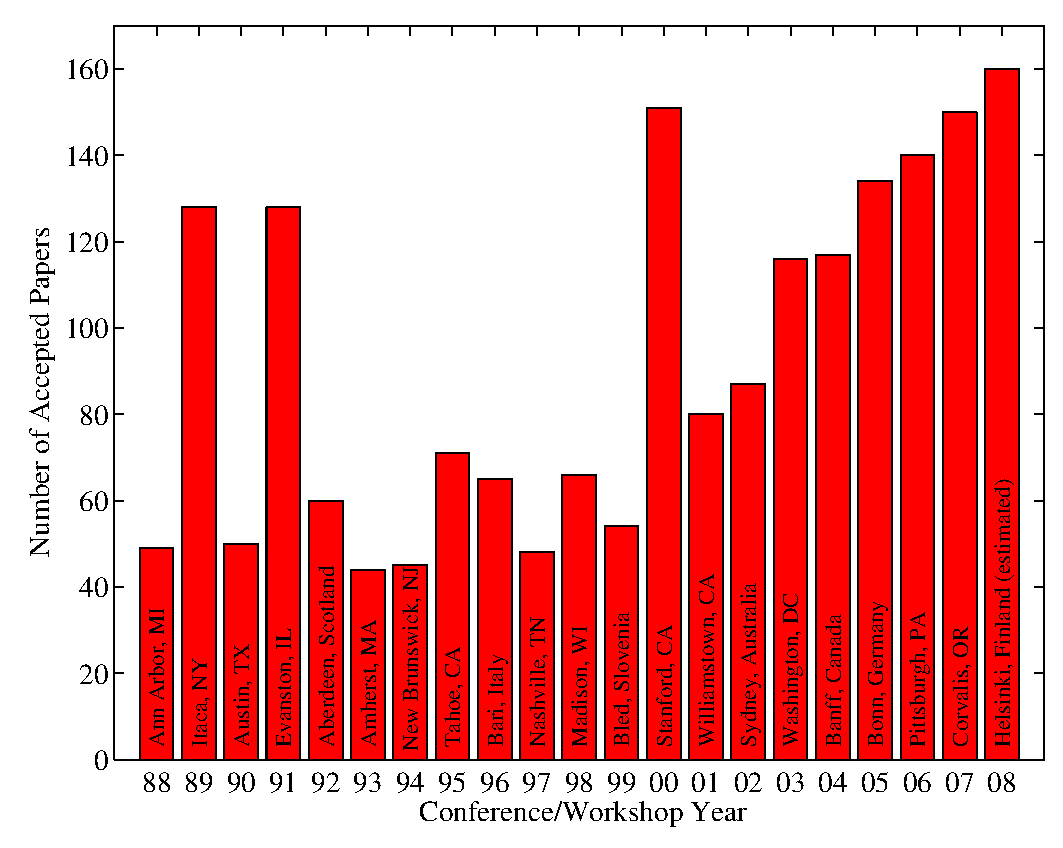
\includegraphics[width=\columnwidth]{icml_numpapers}}
% \caption{Historical locations and number of accepted papers for International
% Machine Learning Conferences (ICML 1993 -- ICML 2008) and International
% Workshops on Machine Learning (ML 1988 -- ML 1992). At the time this figure was
% produced, the number of accepted papers for ICML 2008 was unknown and instead
% estimated.}
% \label{icml-historical}
% \end{center}
% \vskip -0.2in
% \end{figure}

\section{Figures}

You may want to include figures in the paper to illustrate your approach and results. Such artwork should be centered, legible, and separated from the text. Lines should be dark and at least 0.5~points thick for purposes of reproduction, and text should not appear on a gray background.

Label all distinct components of each figure. If the figure takes the form of a graph, then give a name for each axis and include a legend that briefly describes each curve. Do not include a title inside the figure; instead, the caption should serve this function.

%Number figures sequentially, placing the figure number and caption \emph{after} the graphics, with at least 0.1~inches of space before

%You may float figures to the top or bottom of a column, and you may set wide figures across both columns (use the environment \texttt{figure*} in \LaTeX). Always place two-column figures at the top or bottom of the page.


% Ejemplo de algoritmo (creo que no usaremos esto)
% \begin{algorithm}[tb]
%    \caption{Bubble Sort}
%    \label{alg:example}
% \begin{algorithmic}
%    \STATE {\bfseries Input:} data $x_i$, size $m$
%    \REPEAT
%    \STATE Initialize $noChange = true$.
%    \FOR{$i=1$ {\bfseries to} $m-1$}
%    \IF{$x_i > x_{i+1}$}
%    \STATE Swap $x_i$ and $x_{i+1}$
%    \STATE $noChange = false$
%    \ENDIF
%    \ENDFOR
%    \UNTIL{$noChange$ is $true$}
% \end{algorithmic}
% \end{algorithm}


% Ejemplo de tabla
% \begin{table}[t]
% \caption{Classification accuracies for naive Bayes and flexible
% Bayes on various data sets.}
% \label{sample-table}
% \vskip 0.15in
% \begin{center}
% \begin{small}
% \begin{sc}
% \begin{tabular}{lcccr}
% \toprule
% Data set & Naive & Flexible & Better? \\
% \midrule
% Breast    & 95.9$\pm$ 0.2& 96.7$\pm$ 0.2& $\surd$ \\
% Cleveland & 83.3$\pm$ 0.6& 80.0$\pm$ 0.6& $\times$\\
% Glass2    & 61.9$\pm$ 1.4& 83.8$\pm$ 0.7& $\surd$ \\
% Credit    & 74.8$\pm$ 0.5& 78.3$\pm$ 0.6&         \\
% Horse     & 73.3$\pm$ 0.9& 69.7$\pm$ 1.0& $\times$\\
% Meta      & 67.1$\pm$ 0.6& 76.5$\pm$ 0.5& $\surd$ \\
% Pima      & 75.1$\pm$ 0.6& 73.9$\pm$ 0.5&         \\
% Vehicle   & 44.9$\pm$ 0.6& 61.5$\pm$ 0.4& $\surd$ \\
% \bottomrule
% \end{tabular}
% \end{sc}
% \end{small}
% \end{center}
% \vskip -0.1in
% \end{table}

\subsection{Citations and References}

Please use APA reference format regardless of your formatter
or word processor. If you rely on the \LaTeX\/ bibliographic
facility, use \texttt{natbib.sty} and \texttt{icml2021.bst}
included in the style-file package to obtain this format.

Citations within the text should include the authors' last names and
year. If the authors' names are included in the sentence, place only
the year in parentheses using yrcite.

Alphabetize references by the surnames of the first authors, with
single author entries preceding multiple author entries. Order
references for the same authors by year of publication, with the
earliest first. Make sure that each reference includes all relevant
information (e.g., page numbers).

Please put some effort into making references complete, presentable, and
consistent. If using bibtex, please protect capital letters of names and
abbreviations in titles, for example, use \{B\}ayesian or \{L\}ipschitz
in your .bib file.


% In the unusual situation where you want a paper to appear in the
% references without citing it in the main text, use \nocite
% \nocite{}

\bibliography{main}
\bibliographystyle{icml2021}


\end{document}

